\chapter{Asking Wealthy Americans How They Got Rich! (Florida)}

This School of Hard Knocks interview, curated by LazyingArt LLC, is built out of street encounters, but it moves with more discipline than the format first suggests. The lecture spends consequence before cause, then resets the scene statistically, and only after that lets Tampa yield its cases one by one: people before homogenization, diversification across unlike categories, leverage as a capital instrument, time as the irrecoverable asset, self as business and brand, living beneath means, and finally the distinction between paying with labor-time and paying with creativity. There is no board-work here to transcribe, so the formulas below are transcript-led reconstructions of commercial logic. We keep \(Y\) for money made in a year, \(R\) for business revenue, \(T\) for duration, and \(W\) only for cautious reconstructions of wealth state.

\section{Cold Open and Tampa as a Wealth Field}

The lecture begins by spending outcomes before we know whose outcomes they are. We hear fragments of scale, risk, and financing before Tampa has even been named:
\begin{equation}
Y_{\text{teaser},1} > \$10\,\text{million},\qquad
Y_{\text{teaser},2} \approx \$15\,\text{million},\qquad
L_{\text{teaser}} = \$550{,}000.
\end{equation}
These opening quantities are not yet an argument. They are bait. The lecture wants us to feel the size of the prizes and the size of the bets before it tells us why this city, or these speakers, matter.

One teaser fragment is unstable. The splice seems to contain a \(\$45\) million line, but when the later interview arrives in full, the coherent figure is much smaller and much cleaner:
\begin{equation}
Y_{\text{digital,current}} \approx \$4\text{--}5\,\text{million/year}.
\end{equation}
We should therefore treat the cold open as a collage, not as a settled numerical introduction.

Only after this does the host reset the frame and tell us why Tampa has been chosen:
\begin{equation}
N_{\text{millionaires}} > 60{,}000,\qquad
N_{\text{billionaires}} \approx 10.
\end{equation}
The point of these city counts is methodological. They justify the street-interview form itself. If a city contains wealth at this density, then moving through its expensive districts and stopping operators becomes, in the lecture's own logic, a way of extracting rules directly from the environment.

That is the first rhythm of the chapter. First we are shown consequences. Then we are given a field in which those consequences may be searched. Only then do the interviews begin.

\section{The Older Serial Entrepreneur: People, Diversification, and the Cash Call}

The first full case belongs to an older entrepreneur whose background spans television and restaurants. But the lecture does not begin with his revenue. It begins with his management doctrine. He says the great lesson of entrepreneurship is to take care of one's people, and that the worst thing is to let a large corporation take over and homogenize everything. The reason is not abstract. In his account, homogenization fails because the new regime does not care about the staff.

This ordering matters. The lecture wants the human variable on the table before it lets money enter. Only then does it introduce scale:
\begin{equation}
R_{\text{TV}} \approx \$30\text{--}40\,\text{million/year},\qquad
R_{\text{restaurant}} \approx \$5\,\text{million/year}.
\end{equation}
These are operating revenues, not personal income. The speaker is telling us how large the businesses became, not simply how rich he became.

The next move is equally deliberate. Once staff and scale are both established, the lecture turns to resilience. He says that he always tried to maintain three sources of income:
\begin{equation}
N_{\text{income sources}} = 3,
\end{equation}
and the point is not mere plurality, but categorical separation:
\begin{equation}
\{\text{television},\ \text{restaurant},\ \text{farming}\},
\qquad
\text{category}_i \neq \text{category}_j \quad (i\neq j).
\end{equation}
We should not read this as a slogan about scattered attention. It is a statement about correlated risk. Three businesses in one category may fail together; three businesses in distinct categories need not.

\subsection{Question \& Answer}

\paragraph{Question.} Why diversify across distinct businesses if many entrepreneurs preach concentration?

\paragraph{Answer.} Because the lecture is no longer talking about early-stage focus. It is talking about durability. The older entrepreneur is arguing that wealth becomes fragile when all exposures are tied to one sector, one taste cycle, or one revenue machine. Television, restaurants, and farming are valuable here not simply because they are three lines of business, but because they are three different ways of being wrong. The categories do not rise and fall for exactly the same reasons.

Only after diversification is defended does the lecture widen into biography. The entrepreneur says he grew up on a farm, and when asked about the turning point toward financial freedom, he points back to his father, who took risk every day. In other words, risk appetite is not narrated as a fashionable trait. It is narrated as a learned way of standing in the world.

The age marker is then used almost theatrically:
\begin{equation}
a_{\text{older}} \approx 69,\qquad
a_{\text{older,next}} = 70.
\end{equation}
The host is visibly surprised. That surprise performs a small function in the lecture. It tells us that the advice now coming is being heard as long-tested advice.

The next piece is one of the cleanest business screens in the entire episode. Any business, he says, will need additional cash flow at some point. Partners will be tested when that moment arrives. If we denote the required infusion by \(C_{\text{call}}\), the rule becomes
\begin{equation}
\text{partner can meet } C_{\text{call}}
\;\Rightarrow\;
\text{partner survives the stress test},
\end{equation}
\begin{equation}
\text{partner cannot meet } C_{\text{call}}
\;\Rightarrow\;
\text{that person should not be your partner}.
\end{equation}
This is not finance in textbook dress. It is operator logic. But it is sharp. The lecture is saying that partnership should be judged under stress, not under enthusiasm.

The section closes by cashing in one of the very first teaser fragments. In a different banking era, he says, he walked into a bank on a Saturday, met the president on his day off, and opened his first business with
\begin{equation}
L_{\text{first business}} = \$550{,}000.
\end{equation}
The point is not merely historical color. It ties together the whole first case: people, risk, diversification, partnership, and credit all belong to one operating picture.

The host then performs the lecture's first explicit recap. He says, in effect, that it all comes back to people, and that people can take us places money cannot. That recap is not decorative. It is the hinge that lets the lecture pivot, in the next encounter, away from people and toward leverage.

\section{The Younger Investor: Leverage Debt and Choose Your Hard}

After the first recap, the lecture abruptly changes temperature. The next speaker is younger, operates in digital marketing, and says he has been an entrepreneur only for
\begin{equation}
T_{\text{digital}} \approx 3\text{--}4\ \text{years},
\end{equation}
yet is already making
\begin{equation}
Y_{\text{digital,current}} \approx \$4\text{--}5\,\text{million/year}.
\end{equation}
This change of generation is important. We have just heard an older operator explain people, categories, and partner discipline. Now the lecture turns to capital structure.

His advice is stated immediately: leverage debt. The first part of his claim is polemical. Many people, he says, are trying to get out of debt, but that only moves them from negative to broke. In compact form,
\begin{equation}
W<0 \;\to\; W=0
\end{equation}
is not yet a theory of wealth creation. It is only the cancellation of a deficit.

The positive theory comes next. One uses other people's money to acquire something that throws off cash flow. That is the mechanism. Since no validated diagram survives from the lecture, the figure below is an editorial compression of the spoken sequence rather than a redraw of a seen board.

\begin{figure}[h]
\centering
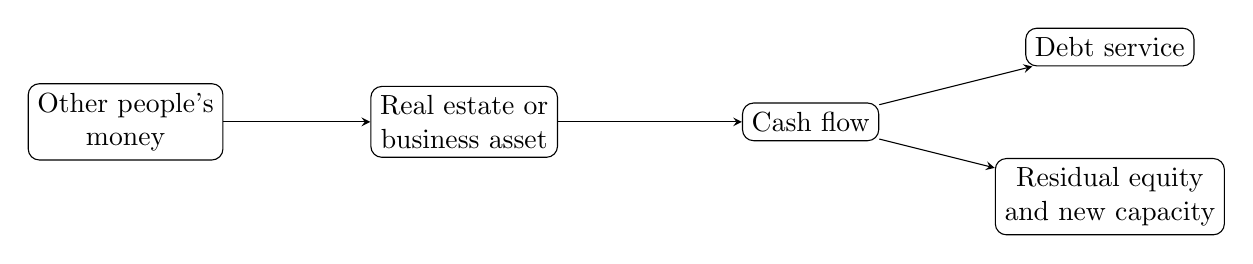
\begin{tikzpicture}[>=stealth]
\node[draw, rounded corners, align=center] (a) at (0,0) {Other people's\\money};
\node[draw, rounded corners, align=center] (b) at (4.3,0) {Real estate or\\business asset};
\node[draw, rounded corners, align=center] (c) at (8.7,0) {Cash flow};
\node[draw, rounded corners, align=center] (d) at (12.5,0.95) {Debt service};
\node[draw, rounded corners, align=center] (e) at (12.5,-0.95) {Residual equity\\and new capacity};
\draw[->] (a)--(b);
\draw[->] (b)--(c);
\draw[->] (c)--(d);
\draw[->] (c)--(e);
\end{tikzpicture}
\caption{Transcript-derived leverage loop from the younger entrepreneur's explanation.}
\end{figure}

In symbolic shorthand, we may write
\begin{equation}
\text{OPM}
\;\to\;
\text{asset purchase}
\;\to\;
\text{cash flow}
\;\to\;
\text{debt repayment},
\end{equation}
where \(\text{OPM}\) is only note-writer shorthand for ``other people's money.''

\paragraph{Worked reconstruction.} If the acquired asset generates periodic cash flow \(F\) and the required debt service is \(D\), then the logic of the lecture is that the arrangement is constructive only when
\begin{equation}
F>D.
\end{equation}
Under that condition the retained wealth update is
\begin{equation}
W_{n+1}=W_n+(F-D).
\end{equation}
This algebra is our own cleaned version of the spoken argument, not the speaker's notation. But it preserves the key point exactly: the debt is useful only if the borrowed capital sits in front of a machine that pays more than it consumes.

\subsection{Question \& Answer}

\paragraph{Question.} How can debt function as a wealth-building tool rather than merely as a liability?

\paragraph{Answer.} In the lecture's terms, debt becomes a tool only when it is placed in front of cash flow. Borrowing to consume is merely delayed impoverishment. Borrowing to acquire a property or a business whose inflow exceeds its debt service changes the structure completely. Now debt is not the thing to be feared in isolation; the real question is what kind of asset stands behind it. That is why the speaker says that people who never learn leverage end up working for those who do.

Having made this financial point as sharply as possible, the lecture immediately refuses to let it remain abstract. The speaker says he went to college for only
\begin{equation}
T_{\text{college}} \approx 90\ \text{days},
\end{equation}
and became a millionaire at about
\begin{equation}
a_{\text{millionaire}} \approx 27.
\end{equation}
He also describes a violent instability in early life: father dead when he was a child, mother jailed for a period. These details are not side material. They restore the motivational texture that a purely financial summary would lose.

That is why the section does not end on debt. It ends on hardship. Starting a business is hard; investing is hard; repairing credit is hard. But being broke, or standing in the same place year after year, is also hard. The lecture compresses the contrast into a pair of rival burdens:
\begin{equation}
\text{hard}_{\text{build/invest/repair}}
\qquad \text{vs.} \qquad
\text{hard}_{\text{stay broke/stagnate}}.
\end{equation}
Once that line has been spoken, the lecture is ready for a genuine interruption. It widens from money to time.

\section{Sponsor Interruption: Time as the Scarce Asset}

The sponsor block matters structurally because it is not merely inserted; it is motivated. The host says that after interviewing a large number of wealthy people, the greatest lesson is that time is the asset one never gets back. That claim is then monetized through the CookUnity segment.

The numbers here should be recorded, but they belong to a different layer of the lecture:
\begin{equation}
N_{\text{millionaires interviewed}} > 1000,\qquad
d_{\text{CookUnity}} = 50\%.
\end{equation}
Just before the next interview, the host also advertises the size of his own channel:
\begin{equation}
N_{\text{followers}} = 8\,\text{million},\qquad
V_{\text{monthly views}} \approx 170\,\text{million/month}.
\end{equation}
These figures participate in the lecture's rhetoric of credibility and scale, but they do not replace the entrepreneurial spine of the episode. The important conceptual bridge is simpler: money is no longer the only scarce thing on the page; time has now been named as the deeper cost.

\section{David Bautista: Commodity, Brand, and Living Beneath Means}

With David Bautista, the lecture changes register again, moving from local operators to entertainment. But it keeps the business spine intact. He says he has been in entertainment for roughly
\begin{equation}
T_{\text{Bautista}} \approx 25\ \text{years},
\end{equation}
and has earned more than
\begin{equation}
Y_{\text{Bautista,max}} > \$10\,\text{million/year}.
\end{equation}
As before, however, the endpoint is immediately tied to a harsh beginning: a single mother, periods without enough food, the worst parts of Washington, D.C., and no real money until well into his thirties:
\begin{equation}
T_{\text{Bautista,no money}} \approx \text{until well into his 30s}.
\end{equation}
The lecture keeps insisting on this pattern. Wealth is not allowed to float free of delay, failure, or hardship.

The first decisive lesson in this segment comes from Triple H. Bautista says that when he first entered wrestling, he was too worried about hierarchy, about offense, about making enemies. The mentor's correction was brutal and simple: this is a business. We may compress the doctrine as
\begin{equation}
\text{self} = \text{business} = \text{commodity} = \text{brand}.
\end{equation}
This is a useful compression so long as we remember what it is doing. It is not trying to say that a person is nothing but a brand. It is saying that once income depends on the self as a public object, one must make decisions in commercial rather than purely emotional terms.

A second mentor lesson is even more concrete. The Undertaker's rule, passed down from his father, is to live beneath one's means. In the cleanest notation,
\begin{equation}
C<Y,\qquad S=Y-C>0,
\end{equation}
where \(C\) is consumption, \(Y\) income, and \(S\) the retained surplus. This is one of the lecture's simplest formulas, but it carries a great deal of weight. Bautista says he learned it the hard way: after wrestling, he lost everything and even had his house foreclosed on. The second chance came only later, in film.

If the surplus \(S\) persists year after year, then even without modelling return on capital we have the elementary update rule
\begin{equation}
W_n=W_0+nS.
\end{equation}
That is already enough to explain the lecturer's tone. ``Live beneath your means'' is not functioning here as moral advice. It is functioning as a structural way of preserving optionality after success has already arrived.

\subsection{Question \& Answer}

\paragraph{Question.} Why does living beneath one's means remain rational even after very large earnings?

\paragraph{Answer.} Because the lecture refuses to identify high income with durable position. Bautista's own story is the proof inside the lecture: large success arrived, then collapse arrived, and only then did a second career become possible. Once we keep that sequence in view, the inequality \(C<Y\) no longer sounds like asceticism. It becomes a way of storing room to move when the first machine shuts down.

That is why the Bugatti example lands so cleanly:
\begin{equation}
P_{\text{Bugatti}} \approx \$3\text{--}5\,\text{million}.
\end{equation}
He is not saying that luxury is forbidden. He is saying that the object is unnecessary, and that unused cash has become more valuable to him than one more visible indulgence.

The section then makes one last hard turn. In a competitive entertainment machine, Bautista says, we cannot expect to like everybody with whom we do business. The relevant screen is not friendship but mutual commercial usefulness. This resolves a tension that has been building through the chapter: social approval is not the same thing as strategic position.

The host's recap makes the point even sharper. If we enter business expecting to be liked by everybody, we will not succeed. That recap clears the way for the final interview, where the lecture moves from brand discipline to its most abstract wealth distinction.

\section{The Final Consultant: Paying with Time, Paying with Creativity}

Only now does the lecture fully cash in the very first cold-open voice. We return to the consultant with the Rolls Royce, and the teaser fragments acquire their owner. He says he has been a business owner for
\begin{equation}
T_{\text{final}} = 39\ \text{years},
\end{equation}
and that the most money he has made in a single year is roughly
\begin{equation}
Y_{\text{final,max}} \approx \$15\,\text{million/year}.
\end{equation}
When asked whether he has been broke, he does not answer with a single episode. He gives a sequence:
\begin{equation}
W_{\text{broke}}
\to
W_{\text{millions}}
\to
W_{\text{broke again}}
\to
W_{\text{stabilized}}.
\end{equation}
This is a fitting final case because it gathers several recurring motifs at once. Wealth can rise, collapse, and be rebuilt. High income is not the same thing as permanent safety. Time and structure still matter.

Then comes the lecture's most compressed abstraction. Poor and middle-class people, he says, experience things as expensive because they pay for them with money exchanged directly for time, and therefore with life. Wealthy entrepreneurs pay differently. They pay according to creativity; they create an offer that pays for what they buy. In cleaned form,
\begin{equation}
\text{purchase}_{\text{poor/middle}}
\sim t_{\text{labor}},
\qquad
\text{purchase}_{\text{wealthy entrepreneur}}
\sim c_{\text{creative offer}}.
\end{equation}
We should not literalize the slogan that ``everything costs the same amount.'' The mathematically honest reading is the contrast above. The speaker is distinguishing payment mechanisms, not denying price differences.

\subsection{Question \& Answer}

\paragraph{Question.} What does it mean to pay for things with creativity rather than with time?

\paragraph{Answer.} It means that the entrepreneur is not confined to the sequence
\[
\text{hours} \to \text{wages} \to \text{purchase}.
\]
Instead he creates a structure, an offer, a deal, or a commercial arrangement that generates the means of payment. That is the sense in which creativity becomes the operative currency. The claim is intentionally provocative, but it should remain speaker-attributed and heuristic. The lecture is offering a contrast in economic posture, not a literal theorem of pricing.

After its most abstract commercial line, the lecture makes one final turn, from entrepreneurship to spiritual filtration. The consultant says he does not merely believe in God; he trusts God. He received Christ at
\begin{equation}
a_{\text{received Christ}} = 16,
\end{equation}
began reading the Bible at
\begin{equation}
a_{\text{began Bible reading}} = 17,
\end{equation}
and then gives the rule by which he handles every later success principle: if it aligns with Scripture, he follows it; if it does not, he drops it. The chapter ends, therefore, not with a maximization problem, but with a filter. Even success doctrine must answer to something prior.

\section{Summary}

The lecture begins by showing us outcomes before it explains them, and that consequence-first structure governs everything that follows. Tampa is presented as a concentrated wealth field; the older entrepreneur turns that field into doctrine about people, diversification, and partner quality; the younger investor shifts us into leverage and the use of other people's money; the sponsor block widens the discussion from money to time; Bautista translates celebrity back into business structure through brand discipline and low consumption; and the final consultant closes by contrasting labor-time payment with creativity-backed offers.

What gives the chapter its coherence is not one master formula, but a repeated motion from visible sign to underlying mechanism. The Rolls Royce is not the lesson; the capital structure behind it is. The celebrity is not the lesson; the brand discipline and stored optionality are. The annual income is not the lesson; the wealth path that survives collapse is. If we preserve that movement, then the lecture unfolds as it should: not as a bag of quotes, but as a guided sequence from anecdote, to number, to mechanism, and then onward to the next case.